\graphicspath{ {project_images/} }

\section{Methods}

The SVM, ResNet50, CNN, and VGG16 classifiers were implemented for our project. We also experimented with CLIP to learn about how the model approached image classification.

\subsection{SVM}

\subsection{ResNet50}

\subsection{CNN}
Convolutional Neural Networks (CNN) is commonly used for image classification tasks. Typically, CNN models consist of convolutional layers that apply filters to extract features and patterns, pooling layers to retain the important features and patterns, and fully connected layers to make predictions based on the features learned in the convolutional and pooling layers.
Our CNN model implements a sequential structure, where the layers are added linearly. The input layer takes in the parameters of the image, in our case our images were 500x500 pixels with a color channel of 1 (since they are greyscale images). After input, the first convolutional layer applies filters to capture the features in the image data by moving a matrix of learnable weights over the image. In our model, the filters had a size of 3x3 and the number of filters increased in each convolutional layer. At the beginning of training, the weights are random before adapting its value throughout the training process. The extracted features are put into a feature map that the following pooling layer uses to further extract important features. Our model uses max-pooling, which looks for the maximum value extracted by each filter from the previous layer so that the initial feature map is downsampled. This pattern of convolutional layer followed by pooling layer iterates to continue extracting features and downsampling the feature map before a flatten layer reshapes the feature map into a one-dimensional vector that can be inputted into a fully connected dense layer. The convolutional layers and max-pooling layers iterate 3 times in our model before the feature map is flattened. We found that less iterations yielded poorer performance (model was not complex enough) and more iterations resulted in longer training time (model was more complex and computational load was larger). The dense layer is considered a "fully connected" layer because each neuron in a dense layer is connected to every extracted feature and is assigned a weight value. The initial weights are random but are learned throughout the training process. The weight of each of the connections in the dense layer attempt to understand the relationship between the important features extracted from the previous layers as a representation of a prominent feature. The output layer is a dense layer with neurons equal to the number of classes in the dataset; in our case there are 3 classes (cat, dog, and panda). The summary of the structure of our CNN model is shown in Figure \ref{fig:figure1} below.

\begin{figure}[h]
	\centering
	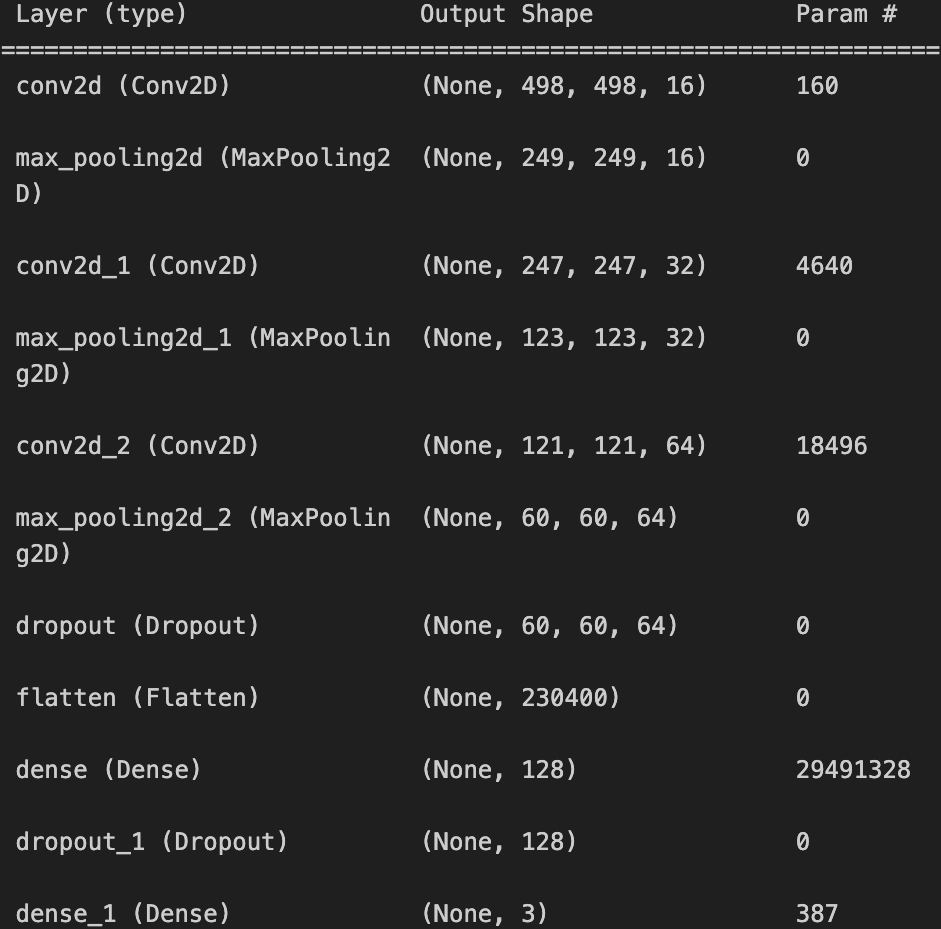
\includegraphics[scale=0.5]{CNN_structure}
	\caption{CNN model summary.}
	\label{fig:figure1}
\end{figure}

Our convoluted layers use the Rectified Linear Unit (ReLu) activation function to introduce non-linearity, this way our model can learn complex relationships between the features of our data. The ReLu activation function sets negative values found in the convolution matrix to 0, allowing the model to focus on the positive values that likely represent relevant features. The output dense layer uses the Softmax activation function to scale the numerical output of the model into probabilities distributed over the possible output classes represented by indexes. The class with the highest probability is considered the predicted class which is mapped to the string value of the class using the index value. 

\subsection{VGG16}